\documentclass[11pt,a4paper]{article}
\usepackage[T1]{fontenc}
\usepackage[utf8]{inputenc}
\usepackage{lmodern}
\usepackage[margin=23mm,headheight=15pt]{geometry}
\usepackage{amsmath,amssymb,amsfonts,mathtools,bm}
\usepackage{booktabs,longtable,tabularx,array}
\usepackage{graphicx,xcolor}
\usepackage{tikz}
\usetikzlibrary{arrows.meta,positioning,shapes.geometric,fit,calc}
\usepackage{listings}
\usepackage{enumitem}
\usepackage{microtype}
\usepackage{hyperref}
\usepackage{fancyhdr}
\usepackage{tcolorbox}
\tcbuselibrary{breakable}
\usepackage{titlesec}
\usepackage{caption}
\usepackage{float}
\usepackage{siunitx}
\definecolor{navy}{HTML}{123154}
\definecolor{teal}{HTML}{15747B}
\definecolor{pale}{HTML}{F2F7FA}
\definecolor{codebg}{HTML}{F7F8FA}
\definecolor{commentgreen}{HTML}{41754F}
\definecolor{codepurple}{HTML}{613F80}
\hypersetup{colorlinks=true,linkcolor=navy,urlcolor=teal,citecolor=navy,pdftitle={Marlin FFT Mechanics: A Guide for FEM Users},pdfauthor={Technical tutorial based on the public Marlin application}}
\titleformat{\section}{\Large\bfseries\color{navy}}{\thesection}{0.7em}{}
\titleformat{\subsection}{\large\bfseries\color{navy}}{\thesubsection}{0.7em}{}
\setlength{\parskip}{0.43em}
\setlength{\parindent}{0pt}
\setlist[itemize]{topsep=3pt,itemsep=2pt,parsep=0pt}
\setlist[enumerate]{topsep=3pt,itemsep=3pt,parsep=0pt}
\pagestyle{fancy}
\fancyhf{}
\fancyhead[L]{\footnotesize\color{navy} MARLIN | FFT-based mechanics}
\fancyhead[R]{\footnotesize FEM-to-FFT tutorial}
\fancyfoot[C]{\thepage}
\newcommand{\avg}[1]{\left\langle #1\right\rangle}
\newcommand{\dd}{\mathrm{d}}
\newcommand{\Grad}{\operatorname{Grad}}
\newcommand{\Div}{\operatorname{Div}}
\newcommand{\sym}{\operatorname{sym}}
\newcommand{\mb}[1]{\boldsymbol{#1}}
\newcommand{\code}[1]{\texttt{\detokenize{#1}}}
\newtcolorbox{keybox}[1][]{colback=pale,colframe=teal!55!black,boxrule=0.55pt,arc=1.5mm,breakable,#1}
\newtcolorbox{warnbox}[1][]{colback=yellow!5,colframe=orange!70!black,boxrule=0.55pt,arc=1.5mm,breakable,#1}
\lstdefinestyle{input}{basicstyle=\ttfamily\footnotesize,backgroundcolor=\color{codebg},frame=single,rulecolor=\color{black!18},breaklines=true,breakatwhitespace=false,columns=fullflexible,keepspaces=true,showstringspaces=false,commentstyle=\color{commentgreen},keywordstyle=\color{codepurple},morecomment=[l]{\#},xleftmargin=3pt,xrightmargin=3pt,aboveskip=7pt,belowskip=7pt}
\lstdefinestyle{shell}{style=input,basicstyle=\ttfamily\small}
\renewcommand{\arraystretch}{1.17}
\begin{document}
\pagenumbering{roman}
\begin{titlepage}
\vspace*{20mm}
{\color{teal}\rule{\textwidth}{2.5pt}}\\[13mm]
{\Huge\bfseries\color{navy} Marlin: Solving Solid Mechanics\\[3mm] with the Fast Fourier Transform}\par
\vspace{11mm}
{\Large A detailed, FEM-oriented introduction to the numerical method, solver architecture, and input-file syntax}\par
\vspace{14mm}
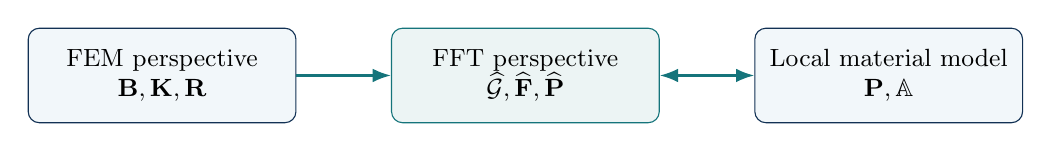
\begin{tikzpicture}[>=Latex, node distance=7mm, every node/.style={font=\small}]
\node[draw=navy,rounded corners,fill=pale,minimum width=3.4cm,minimum height=1.2cm,align=center] (fem) {FEM perspective\\\(\mathbf{B},\mathbf{K},\mathbf{R}\)};
\node[draw=teal,rounded corners,fill=teal!8,minimum width=3.4cm,minimum height=1.2cm,right=12mm of fem,align=center] (fft) {FFT perspective\\\(\widehat{\mathcal G},\widehat{\mathbf F},\widehat{\mathbf P}\)};
\node[draw=navy,rounded corners,fill=pale,minimum width=3.4cm,minimum height=1.2cm,right=12mm of fft,align=center] (material) {Local material model\\\(\mathbf P,\mathbb A\)};
\draw[->,thick,teal] (fem)--(fft);
\draw[<->,thick,teal] (fft)--(material);
\end{tikzpicture}
\vfill
{\large Source-aligned technical tutorial}\par
{\normalsize Public repository: \url{https://github.com/idaholab/marlin}}\par
{\normalsize Documentation: \url{https://marlin.inl.gov/}}\par
{\normalsize Prepared 13 October 2026}\par
\vspace{5mm}
{\footnotesize This is an independent explanatory tutorial, not an official Marlin manual. Details of custom/local extensions must be checked against their source.}
\end{titlepage}
\tableofcontents
\clearpage
\pagenumbering{arabic}

\section{Executive orientation: what is Marlin?}
Marlin is a Fourier/spectral solver application built in the MOOSE ecosystem. Rather than creating the global finite-element stiffness matrix on an unstructured mesh, it stores fields on a \emph{regular Cartesian grid} and uses discrete Fourier transforms to evaluate spatially coupled operators. LibTorch supplies array operations and Fourier transforms, including CPU/GPU paths. Marlin still uses MOOSE input-file syntax, execution infrastructure, and optional coupling facilities.

\begin{keybox}
\textbf{The central idea:} FFT is not a new material law. It is a different numerical way of enforcing equilibrium and compatibility over a regular, usually periodic, microstructural cell. At each grid cell, the constitutive model still calculates stress and a tangent from the local deformation state.
\end{keybox}

For solid mechanics two solver families should not be conflated:
\begin{itemize}
\item \code{FFTMechanics}: heterogeneous \emph{finite-strain} variational FFT mechanics, following the Newton--conjugate-gradient approach of de Geus \emph{et al.} (2017). This is the primary focus of this guide and is a plausible basis for a custom crystal-plasticity model.
\item \code{FFTQuasistaticElasticity}: a separate, \emph{homogeneous linear} elasticity calculation in Fourier space with a concentration/eigenstrain forcing. It is not a generic replacement for the heterogeneous nonlinear solver.
\end{itemize}
These statements and the input parameter names are based on the public Marlin repository and documentation [\ref{sec:references}].

\section{Translate familiar FEM concepts into FFT concepts}
\begin{table}[H]\centering\small
\begin{tabularx}{\textwidth}{@{}p{0.33\textwidth}X@{}}\toprule
\textbf{In FEM} & \textbf{In periodic FFT mechanics}\\\midrule
Geometric elements and quadrature points & Uniform pixels/voxels and regularly sampled field values\\
Nodal displacement unknowns $\mathbf u_a$ & Periodic fluctuation field, represented by Fourier modes or compatible deformation-gradient samples\\
Strain-displacement matrix $\mathbf B$ & Spectral differentiation / Fourier-space compatibility projector $\widehat{\mathcal G}$\\
Element loop and assembly & Local array operations plus FFT/inverse FFT; no conventional assembled global FEM stiffness matrix\\
Residual $\mathbf R=\mathbf f_{\rm int}-\mathbf f_{\rm ext}$ & Projected stress field $\mathcal G:\mathbf P$, representing equilibrium residual\\
Tangent stiffness $\mathbf K=\partial\mathbf R/\partial\mathbf u$ & Matrix-free operator $\delta\mathbf F\mapsto \mathcal G:(\mathbb A:\delta\mathbf F)$\\
Newton + sparse linear solver & Nonlinear iterations + FFT-based matrix-free linear solve (CG in current \code{FFTMechanics})\\
Dirichlet/Neumann boundary faces & Commonly prescribed \emph{average} deformation and periodic fluctuation constraints\\
Material integration at quadrature points & Material update independently at each voxel\\
Exodus field visualization & Grid tensor outputs (e.g. XDMF/HDF5) and optional mesh projections\\\bottomrule
\end{tabularx}
\caption{A conceptual mapping, not a statement that the two discretizations are identical.}
\end{table}

\section{Start from the exact same mechanics equations}
\subsection{Small-strain mechanics: the FEM form you know}
For a linearly elastic body without body forces,
\begin{equation}
\nabla\cdot\mb\sigma=\mathbf 0,\qquad
\mb\varepsilon=\sym\nabla\mathbf u,\qquad
\mb\sigma=\mathbb C(\mathbf x):\mb\varepsilon.
\end{equation}
The FEM weak statement is $\int_\Omega\nabla^s\mathbf v:\mb\sigma\,\dd V=0$ for all admissible test functions. Discretization produces $\mathbf R(\mathbf u)=\mathbf0$, and Newton's method uses the tangent system $\mathbf K\Delta\mathbf u=-\mathbf R$.

The FFT method solves the \emph{same local balance law}. The change is the representation of derivatives and compatible trial/test fields: trigonometric Fourier modes on a regular grid instead of piecewise finite-element shape functions on an arbitrary mesh.

\subsection{Finite strain: the form relevant to \code{FFTMechanics}}
Use reference coordinates $\mathbf X$ and define
\begin{equation}
\mathbf F=\frac{\partial\mathbf x}{\partial\mathbf X}=\mathbf I+\Grad\mathbf u,
\qquad \Div\mathbf P=\mathbf0,
\qquad \mathbf P=\mathcal P(\mathbf F,\mb\alpha),
\label{eq:finitebalance}
\end{equation}
where $\mathbf P$ is first Piola--Kirchhoff stress and $\mb\alpha$ denotes optional material internal variables (slip resistance, dislocation density, etc.). The physically work-conjugate pair for a total-Lagrangian formulation is $(\mathbf P,\mathbf F)$.

For a periodic RVE the deformation is decomposed into an affine part and periodic fluctuations:
\begin{equation}
\mathbf u(\mathbf X)= (\overline{\mathbf F}-\mathbf I)\mathbf X+\widetilde{\mathbf u}(\mathbf X),
\quad \widetilde{\mathbf u}\ \text{periodic},\quad
\avg{\Grad\widetilde{\mathbf u}}=\mathbf0.
\label{eq:split}
\end{equation}
Consequently $\mathbf F(\mathbf X)=\overline{\mathbf F}+\Grad\widetilde{\mathbf u}$ and $\avg{\mathbf F}=\overline{\mathbf F}$. Opposite-face fluctuation fields are periodic and nominal tractions are anti-periodic. An overall displacement translation must be fixed by convention; it does not change $\mathbf F$.

\begin{warnbox}
\textbf{Boundary-condition limitation.} The standard periodic spectral formulation does \emph{not} impose an arbitrary dog-bone free surface, one fixed grip, and a displacement on the other grip just by changing \code{[Domain]}. A full tensile specimen with non-periodic external boundaries is usually more naturally treated by FEM, or through a carefully validated FFT--FEM coupling/alternative formulation. For grain-boundary localization, distinguish a \emph{periodic polycrystalline RVE} from a true tensile specimen.
\end{warnbox}

\section{What the Fourier transform does: a first-principles explanation}
\subsection{Represent a field as periodic waves}
In one dimension over a periodic interval of length $L$, sampled on $N$ equally spaced points $x_n=nL/N$, the discrete Fourier transform is
\begin{align}
\widehat f_m &=\sum_{n=0}^{N-1} f_n\,\exp\left(-2\pi i\frac{mn}{N}\right),\\
f_n&=\frac1N\sum_{m=0}^{N-1}\widehat f_m\,\exp\left(2\pi i\frac{mn}{N}\right).
\end{align}
The integer mode number $m$ represents a wave with physical angular wave number $q_m=2\pi m/L$, with the usual wrapped negative-frequency indexing above the Nyquist frequency.

For a wave $f(x)=\sin(2\pi x/L)$, we have $f'(x)=(2\pi/L)\cos(2\pi x/L)$. In Fourier space the \emph{whole derivative} is computed by multiplying each Fourier coefficient by $i q_m$:
\begin{equation}
\boxed{\quad \widehat{\partial_j f}(\mathbf q)=i q_j\widehat f(\mathbf q).\quad}
\label{eq:deriv}
\end{equation}
This is why the FFT is attractive for periodic PDEs: spatial differentiation becomes algebraic multiplication in frequency space. FFT is an efficient algorithm to evaluate these transforms, typically requiring $O(N\log N)$ operations rather than a direct dense Fourier transform requiring $O(N^2)$.

\subsection{Two and three dimensions}
For a cuboid of side lengths $(L_x,L_y,L_z)$, a mode is identified by the vector
\begin{equation}
\mathbf q=2\pi\left(\frac{m_x}{L_x},\frac{m_y}{L_y},\frac{m_z}{L_z}\right),
\quad \widehat{\nabla f}=i\mathbf q\widehat f,
\quad \widehat{\nabla\cdot\mathbf v}=i\mathbf q\cdot\widehat{\mathbf v}.
\end{equation}
Marlin's \code{DomainAction} constructs physical-space positions and reciprocal-space wavevectors. The implementation uses Torch FFT operations (real-to-complex transforms when applicable). The physical lengths matter because $q$ depends on $L$: a domain with 32 samples over $2\pi$ is not physically the same as 32 samples over $1$.

\subsection{What happens at zero frequency?}
The $\mathbf q=\mathbf0$ mode is the spatial average. A projector with $|\mathbf q|^{-2}$ is undefined at zero frequency, so the projection is explicitly set to zero there. \emph{This is intentional:} a Fourier projection fixes periodic fluctuations; the prescribed macroscopic deformation is managed separately. The mean displacement is also a freely chosen gauge and is conventionally set to zero.

\subsection{A visual mental model}
\begin{center}
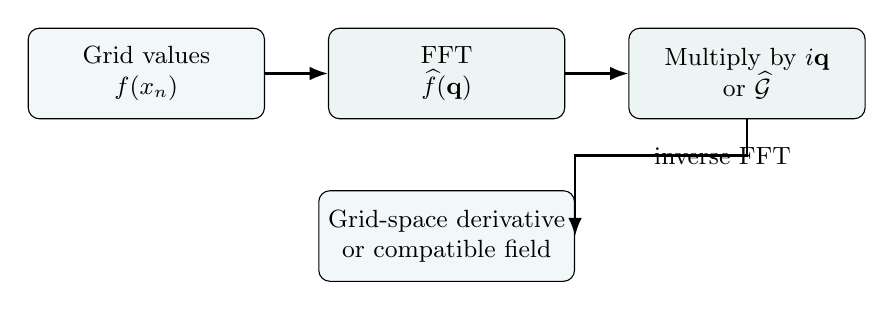
\begin{tikzpicture}[>=Latex,font=\small]
\node[draw,rounded corners,fill=pale,minimum width=3.0cm,minimum height=1.15cm,align=center] (a) {Grid values\\$f(x_n)$};
\node[draw,rounded corners,fill=teal!8,minimum width=3.0cm,minimum height=1.15cm,right=8mm of a,align=center] (b) {FFT\\$\widehat f(\mathbf q)$};
\node[draw,rounded corners,fill=teal!8,minimum width=3.0cm,minimum height=1.15cm,right=8mm of b,align=center] (c) {Multiply by $i\mathbf q$\\or $\widehat{\mathcal G}$};
\node[draw,rounded corners,fill=pale,minimum width=3.0cm,minimum height=1.15cm,below=9mm of b,align=center] (d) {Grid-space derivative\\or compatible field};
\draw[->,thick] (a)--(b);\draw[->,thick] (b)--(c);
\draw[->,thick] (c.south)--++(0,-0.46)-|(d.east) node[pos=.3,right]{inverse FFT};
\end{tikzpicture}
\end{center}
One must distinguish this spatial FFT from a temporal Fourier transform. The loading parameter $t$ in an input file is normally a \emph{load-step/pseudo-time variable}, not a vibration frequency.

\section{From transforms to a solver for heterogeneous equilibrium}
\subsection{Why simply Fourier-transforming a heterogeneous elastic law is not enough}
The constitutive equation is local in position, for example
\begin{equation}
\mb\sigma(\mathbf x)=\mathbb C(\mathbf x):\mb\varepsilon(\mathbf x).
\end{equation}
When $\mathbb C$ changes spatially, the transform of this product is a \emph{convolution}, not simply $\widehat{\mb{\sigma}}=\widehat{\mathbb C}:\widehat{\mb{\varepsilon}}$ pointwise for each mode. Thus one cannot solve each Fourier mode independently for a heterogeneous solid in one algebraic operation.

Instead, typical algorithms alternate between (i) constitutive calculations \emph{in real space}, where each voxel knows its own material, and (ii) spatial projection / solution of the coupled equilibrium problem \emph{using FFTs}.

\subsection{Two important historical routes}
\textbf{Classical Lippmann--Schwinger route.} Choose a homogeneous reference stiffness $\mathbb C^0$, define polarization $\mb\tau=(\mathbb C-\mathbb C^0):\mb\varepsilon$, and employ a Fourier Green operator $\widehat{\mb\Gamma}^0$:
\begin{equation}
\widehat{\mb{\varepsilon}}(\mathbf q)=-\widehat{\mb\Gamma}^0(\mathbf q):\widehat{\mb{\tau}}(\mathbf q),\qquad\mathbf q\ne0,
\end{equation}
with the average strain prescribed separately. This leads to fixed-point or accelerated iterative methods.

\textbf{Variational/Galerkin FFT route.} Treat FFT-based compatibility as a projection in the weak formulation, linearize the constitutive response and solve the resulting tangent problem by a Krylov solver. The Marlin \code{FFTMechanics} implementation follows the finite-strain formulation of de Geus \emph{et al.} and explicitly performs a conjugate-gradient linear solve [\ref{sec:references}]. The implementation is \emph{not} just a simple Lippmann--Schwinger fixed-point scheme.

\subsection{The Fourier compatibility projector}
Suppose $\mathbf A$ is an arbitrary second-order tensor field. In a common continuum index convention, the gradient-compatible part of $\mathbf A$ may be written as
\begin{equation}
\widehat{(\mathcal G:\mathbf A)}_{ij}(\mathbf q)=
\widehat{\mathcal G}_{ijkl}(\mathbf q)\widehat A_{kl}(\mathbf q),\quad
\widehat{\mathcal G}_{ijkl}(\mathbf q)=
\begin{cases}
\displaystyle\delta_{ik}\frac{q_j q_l}{|\mathbf q|^2},&\mathbf q\ne\mathbf0,\\
0,&\mathbf q=\mathbf0.
\end{cases}
\label{eq:proj}
\end{equation}
The literal array index ordering in code can differ by transposes; \emph{the crucial property} is that nonzero Fourier modes are projected onto tensor fields obtainable as gradients of periodic vector fields. Marlin builds a four-index projection tensor from its reciprocal wavevector arrays and then applies it through FFT, tensor contraction, and inverse FFT.

\begin{keybox}
\textbf{Why this enforces equilibrium:} For any compatible fluctuation $\delta\mathbf F=\Grad\delta\widetilde{\mathbf u}$, stationarity of internal work requires $\avg{\mathbf P:\delta\mathbf F}=0$. The projected residual $\mathcal G:\mathbf P$ vanishes precisely in the weak periodic-equilibrium sense represented by the discrete Fourier space. This is analogous to setting every FEM residual component to zero.
\end{keybox}

\section{Nonlinear \code{FFTMechanics}: governing discrete equations}
\label{sec:newton}
\subsection{Discrete variational residual}
For grid values $\mathbf F^a$ and local stresses $\mathbf P^a(\mathbf F^a)$, define the projected residual
\begin{equation}
\mathbf R(\mathbf F)=\mathcal G:\mathbf P(\mathbf F)=\mathbf0.
\label{eq:res}
\end{equation}
The gradient-compatibility space is enforced by $\mathcal G$. Each grid-cell stress is produced \emph{locally} by the constitutive update. In a finite-strain context $\mathbf P$ must be energetically conjugate to $\mathbf F$ (do not silently replace it with Cauchy stress).

\subsection{Newton linearization and matrix-free tangent}
Let
\begin{equation}
\mathbb A_{iJkL}=\frac{\partial P_{iJ}}{\partial F_{kL}}
\end{equation}
be the local constitutive tangent. Linearizing \eqref{eq:res} gives
\begin{equation}
\boxed{\quad\mathcal G:\left[\mathbb A:\Delta\mathbf F\right]
=-\mathcal G:\mathbf P.\quad}
\label{eq:newton}
\end{equation}
The right-hand side is a grid tensor field; the operator on the left is evaluated by (1) applying $\mathbb A$ locally at each voxel and (2) transforming/projecting with FFT. Thus the sparse FEM global stiffness matrix is replaced by an \emph{operator application}. A Krylov algorithm only needs to evaluate \eqref{eq:newton} for trial vectors; it does not need to assemble a dense matrix.

\subsection{What the current public C++ implementation actually does}
The key operations visible in \path{src/tensor_computes/FFTMechanics.C} are:
\begin{enumerate}
\item Construct the reciprocal projector $\widehat{\mathcal G}$ once using $\mathbf q$ and $|\mathbf q|^2$.
\item Initialize the trial deformation-gradient buffer from the existing $\mathbf F$ and evaluate the constitutive model to obtain stress and tangent.
\item Form the incremental macroscopic-deformation forcing if \code{applied_macroscopic_strain} is supplied.
\item Repeatedly call a \emph{conjugate-gradient solver} with the matrix-free operation $\Delta\mathbf F\mapsto\mathcal G:(\mathbb A:\Delta\mathbf F)$.
\item Add the computed correction to the current deformation-gradient tensor, re-evaluate the constitutive model, and form the new projected stress residual $-\mathcal G:\mathbf P$.
\item Stop when its implemented relative/absolute \emph{update norm} tests pass, or report failure when \code{nl_max_its} is exceeded.
\end{enumerate}
The visible implementation computes a relative update as $\|\Delta\mathbf F\|/\|\mathbf F_{\mathrm{initial}}\|$, \emph{not} as a normalized equilibrium residual. Its console output names should therefore not be interpreted as a complete mechanical-equilibrium certificate. For research-grade accuracy, measure $\|\mathcal G:\mathbf P\|$ independently in addition to monitoring the update norm.

\begin{lstlisting}[style=input,caption={Algorithmic pseudocode for the heterogeneous FFT equilibrium solve (not literal Marlin code).}]
Given: periodic grid, F_old, prescribed increment in <F>
Precompute compatible-gradient projector Ghat(q)
Set F_trial from F_old and macroscopic increment
repeat nonlinear iterations:
    (P, A) = constitutive_update(F_trial, state_trial)
    r = -IFFT( Ghat : FFT(P) )
    define MatVec(dF):
        dP = A : dF               # voxel-wise contraction
        return IFFT(Ghat : FFT(dP))
    approximately solve MatVec(dF) = r with a Krylov method
    F_trial = F_trial + dF
    check update AND independently check equilibrium
accept converged F and constitutive state
\end{lstlisting}
\textbf{Important implementation detail:} the actual C++ code includes a particular first-iteration loading correction and ordering of stress/tangent evaluations; use the repository source when debugging the exact iteration. The pseudocode is a conceptual Newton--Krylov view, not a line-by-line reproduction.

\subsection{Why the tangent is essential}
A poor tangent can lead to slow/nonconvergent inner CG iterations even if the stress model is correct. For a custom crystal-plasticity implementation, deriving $\partial\mathbf P/\partial\mathbf F$ is part of the solver interface. The FEM tangent $\partial\mb\sigma/\partial\mb\varepsilon$ is not generally equivalent at finite strain, and a damaged, non-associated, or strongly softening law may produce a nonsymmetric or indefinite tangent for which CG is not guaranteed to work.

\section{What the built-in hyperelastic model computes}
\label{sec:hyper}
The public \code{HyperElasticIsotropic} code uses a Green--Lagrange strain:
\begin{equation}
\mathbf E=\frac12(\mathbf F^T\mathbf F-\mathbf I),\qquad
\mathbf S=\mathbb C:\mathbf E,\qquad
\mathbf P=\mathbf F\mathbf S.
\end{equation}
Here $\mathbf S$ is second Piola--Kirchhoff stress, and the isotropic fourth-order elasticity tensor is generated from $K$ and $\mu$:
\begin{equation}
\mathbb C=K\,\mathbf I\otimes\mathbf I+2\mu\left(\mathbb I_{\rm sym}-\tfrac13\mathbf I\otimes\mathbf I\right),
\qquad\lambda=K-\tfrac23\mu.
\end{equation}
This corresponds to a St.~Venant--Kirchhoff-type hyperelastic model, \emph{not} a crystal-plasticity law and not necessarily a robust model at very large compression/distortion. Its output tangent is consistent with the differentiated first Piola stress $\partial\mathbf P/\partial\mathbf F$.

For orientation, the general material form has the geometric contribution
\begin{equation}
\mathbb A_{iJkL}=\delta_{ik}S_{LJ}+F_{iM}\mathbb C_{MJLN}F_{kN},
\label{eq:tangent}
\end{equation}
when $\mathbb C=\partial\mathbf S/\partial\mathbf E$ has the usual symmetries. The stress field in the test example is \code{stress}; the tangent buffer defaults to \code{dstressdstrain}. The latter name is historical: its \emph{meaning} in this finite-strain solver is the relevant first-Piola/deformation-gradient linearization.

\begin{warnbox}
\textbf{Stress measure and visualization:} The current \code{ComputeVonMisesStress} computes a scalar from the provided \code{stress} buffer. In the example, that buffer holds first Piola stress, not Cauchy stress. A physically interpretable finite-strain von Mises stress should normally be calculated from $\mb\sigma=J^{-1}\mathbf P\mathbf F^T$, with $J=\det\mathbf F$, and then from the deviatoric Cauchy stress. The built-in scalar output must not automatically be reported as Cauchy von Mises stress.
\end{warnbox}

\section{Marlin input-file structure: the main blocks}
\label{sec:syntax}
Marlin uses the familiar MOOSE hierarchical input syntax. The following blocks are the most relevant for mechanics:
\begin{table}[H]\centering\small
\begin{tabularx}{\textwidth}{@{}p{0.26\textwidth}X@{}}\toprule
\textbf{Block} & \textbf{Purpose and FEM analogy}\\\midrule
\code{[Domain]} & Spatial dimension, regular grid, physical extents, FFT layout, and optional mesh device/precision; replaces the numerical role of the FEM \code{[Mesh]} for the spectral calculation.\\
\code{[TensorComputes]}\\ \code{[Initialize]} & Initialize arrays/fields such as phase, $K$, $\mu$, and deformation gradient $\mathbf F$.\\
\code{[TensorComputes]}\\ \code{[Solve]} & Local constitutive model, imposed average loading, coupled nonlinear Fourier-mechanics solve.\\
\code{[TensorComputes]}\\ \code{[Postprocess]} & Convert primary fields into derived output tensors such as displacements and stress invariants.\\
\code{[TensorSolver]} & Calls the root compute for each step/substep; forwards new buffers into the state buffers.\\
\code{[TensorOutputs]} & Writes grid fields such as $\mathbf F$, phase maps, and stresses in XDMF/HDF5.\\
\code{[Executioner]} & Governs steps and the \emph{loading parameter}/time increment, reusing MOOSE infrastructure.\\
\bottomrule\end{tabularx}
\end{table}
Marlin performs dependency resolution among tensor computes. The objects are connected by \emph{named buffers}, not by declarations of elemental residual kernels. A \code{[Domain]} block creates a \code{TensorProblem} automatically if a compatible problem was not explicitly declared.

\section{Annotated mechanics input file: a complete tutorial example}
\label{sec:input}
This example follows the \emph{public Marlin mechanics test's architecture}, but uses a distinct, smooth two-phase modulus field and a small periodic simple-shear demonstration. The full text is also supplied as a separate \code{.i} file with the download. Verify the availability of the test shear helper in your own executable (see warning below).

\begin{lstlisting}[style=input,caption={Annotated demonstration input: \code{marlin_fft_demo.i}.}]
[Domain]
  dim = 2
  nx = 48
  ny = 48
  xmax = ${fparse 2*pi}
  ymax = ${fparse 2*pi}
  mesh_mode = DUMMY
[]

[TensorComputes]
  [Initialize]
    [phase_map]
      type = ParsedCompute
      buffer = phase
      expression = '(0.5+0.5*cos(x))*(0.5+0.5*cos(y))'
      extra_symbols = true
    []
    [bulk_modulus]
      type = ParsedCompute
      buffer = K
      inputs = phase
      expression = 'Km+(Ki-Km)*phase'
      constant_names = 'Km Ki'
      constant_expressions = '1.2 9.6'
    []
    [shear_modulus]
      type = ParsedCompute
      buffer = mu
      inputs = phase
      expression = 'mum+(mui-mum)*phase'
      constant_names = 'mum mui'
      constant_expressions = '0.6 4.8'
    []
    [initial_F]
      type = RankTwoIdentity
      buffer = F
    []
  []

  [Solve]
    [material]
      type = HyperElasticIsotropic
      buffer = stress
      F = Fnew
      K = K
      mu = mu
      tangent_operator = dstressdstrain
    []
    [root]
      [shear_increment]
        type = MacroscopicShearTensor
        buffer = applied_strain
        F = F
      []
      [equilibrium]
        type = FFTMechanics
        buffer = Fnew
        F = F
        K = K
        mu = mu
        constitutive_model = material
        stress = stress
        tangent_operator = dstressdstrain
        applied_macroscopic_strain = applied_strain
        l_tol = 1e-5
        l_max_its = 150
        nl_rel_tol = 1e-4
        nl_abs_tol = 1e-6
        nl_max_its = 80
        verbose = true
      []
    []
  []

  [Postprocess]
    [reconstruct_u]
      type = ComputeDisplacements
      buffer = disp
      F = F
    []
    [scalar_stress_indicator]
      type = ComputeVonMisesStress
      buffer = sV
      stress = stress
    []
  []
[]

[TensorSolver]
  type = ForwardEulerSolver
  root_compute = root
  forward_buffer = F
  forward_buffer_new = Fnew
  substeps = 2
[]

[TensorOutputs]
  [fields]
    type = XDMFTensorOutput
    buffer = 'disp sV F phase'
    output_mode = 'OVERSIZED_NODAL CELL CELL NODE'
    enable_hdf5 = true
    execute_on = 'TIMESTEP_END'
  []
[]

[Executioner]
  type = Transient
  num_steps = 8
  dt = 0.005
[]
\end{lstlisting}

\begin{warnbox}
\textbf{Availability and applicability of the shear helper.} The \code{MacroscopicShearTensor} object is defined under the repository's \code{test/src/tensor_computes/} tree; it is not a general core Marlin loading object. Therefore the tutorial input may require a test-enabled build or inclusion/registration of that source in your local app. The official \code{test/tests/mechanics/mech.i} and \path{examples/degeus_mechanics/mech.i} likewise use test-specific demonstration objects. For your locally developed \code{DDCPAffineLoadTensor}, replace the shear helper only after confirming its registered parameters and compiled implementation. The example here is syntactically source-aligned, not an assertion that every Marlin binary ships with the test helper.
\end{warnbox}

\subsection{Understanding \code{[Domain]} in physical terms}
In the example $L_x=L_y=2\pi$, $N_x=N_y=48$, so $\Delta x=L_x/N_x$ and $\Delta y=L_y/N_y$. The computational domain is topologically periodic. \code{mesh_mode = DUMMY} creates only the auxiliary mesh needed by parts of the MOOSE runtime; \emph{it does not convert the spectral discretization to one FEM element}. The actual mechanics calculation has $48\times48$ grid cells.

The alternative \code{mesh_mode = DOMAIN} creates a matching mesh with one element per grid cell, useful for coupling/visualization. \code{MANUAL} delegates mesh creation to the user. In the public \code{DomainAction} documentation, \code{parallel_mode} includes FFT-specific decomposition options and precision/device choices; these are version sensitive, and distributed execution is specifically flagged as work in progress. Start with a serial CPU validation case.

\subsection{How the phase and elastic constants are assigned}
The \code{phase} field is just a smoothly varying scalar between zero and one. The expressions
\begin{equation}
K(\mathbf x)=K_m+(K_i-K_m)p(\mathbf x),\qquad
\mu(\mathbf x)=\mu_m+(\mu_i-\mu_m)p(\mathbf x)
\end{equation}
produce heterogeneous isotropic elastic moduli. Here subscripts $m$ and $i$ indicate two notional constituents. It is \emph{not} a discrete grain-ID map and carries no crystal orientation. For polycrystalline CP, the corresponding per-voxel data would additionally include grain ID, Euler angles/rotation matrices, phase, and constitutive state.

\subsection{How the solver objects connect}
\begin{center}
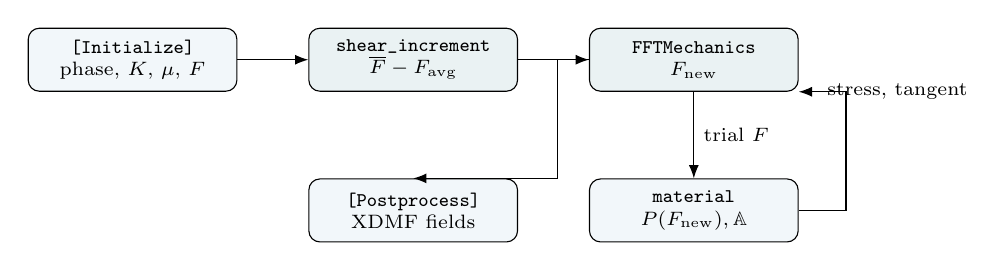
\begin{tikzpicture}[>=Latex,font=\scriptsize,node distance=5mm]
\node[draw,fill=pale,rounded corners,align=center,minimum width=2.65cm,minimum height=.8cm] (phase) {\code{[Initialize]}\\phase, $K$, $\mu$, $F$};
\node[draw,fill=teal!9,rounded corners,align=center,minimum width=2.65cm,minimum height=.8cm,right=9mm of phase] (load) {\code{shear_increment}\\$\overline F-F_{\rm avg}$};
\node[draw,fill=teal!9,rounded corners,align=center,minimum width=2.65cm,minimum height=.8cm,right=9mm of load] (solve) {\code{FFTMechanics}\\$F_{\rm new}$};
\node[draw,fill=pale,rounded corners,align=center,minimum width=2.65cm,minimum height=.8cm,below=11mm of solve] (constit) {\code{material}\\$P(F_{\rm new}),\mathbb A$};
\node[draw,fill=pale,rounded corners,align=center,minimum width=2.65cm,minimum height=.8cm,below=11mm of load] (out) {\code{[Postprocess]}\\XDMF fields};
\draw[->] (phase)--(load);\draw[->] (load)--(solve);
\draw[->] (solve)--node[right]{trial $F$}(constit);
\draw[->] (constit.east)--++(6mm,0)|-node[right,pos=.8]{stress, tangent}(solve.south east);
\draw[->] (solve.west)--++(-4mm,0)|-(out.north);
\end{tikzpicture}
\end{center}
The \code{material} compute returns the named \code{stress} and \code{dstressdstrain} buffers; \code{FFTMechanics} requests it using \code{constitutive_model = material}. Keeping the same names across the consuming and producing objects is essential.

\subsection{What the imposed loading actually means}
The test helper constructs $\overline{\mathbf F}_{\rm target}=\mathbf I+t\,\mathbf e_1\otimes\mathbf e_2$ and returns its difference from the current average of $\mathbf F$. This is a periodic simple-shear \emph{average deformation gradient}, not a prescribed local displacement on the top boundary. The example's \code{dt} and step count control the pseudo-time loading history; ensure the final deformation is what you intend, especially because \code{TensorSolver/substeps} may invoke the mechanics solution more than once per outer step.

\subsection{What is in the output?}
\code{F} is a tensor field stored on spectral grid cells; \code{sV} is a derived scalar stress indicator; \code{phase} is the initially assigned microstructure scalar; \code{disp} is reconstructed from $\mathbf F$ for visualization. \code{ComputeDisplacements} extracts the periodic displacement fluctuation in Fourier space and adds the affine part from the mean $\mathbf F$. Its \code{OVERSIZED_NODAL} grid output is a visualization choice, not an FEM displacement degree of freedom.

For serial tutorial output, \code{XDMFTensorOutput} with \code{enable_hdf5 = true} is appropriate. The public test files use different output restrictions for MPI parallel output (cell mode rather than nodal modes); check your version when switching to distributed FFT execution.

\section{Interpreting the most important solver parameters}
\begin{longtable}{@{}p{0.31\textwidth}p{0.65\textwidth}@{}}\toprule
\textbf{Input parameter} & \textbf{Meaning and practical note}\\\midrule\endfirsthead
\toprule\textbf{Input parameter}&\textbf{Meaning and practical note}\\\midrule\endhead
\code{F}, \code{buffer = Fnew} & Old/current deformation-gradient tensor buffer and newly solved deformation-gradient tensor buffer.\\
\code{constitutive_model} & Name of compute providing the stress and local tangent. Mandatory for \code{FFTMechanics}.\\
\code{stress} & Named stress field (first Piola stress in the demonstrated finite-strain constitutive model).\\
\code{tangent_operator} & Named fourth-order tangent field for the matrix-free Newton--Krylov operator. Default name is \code{dstressdstrain}.\\
\code{K}, \code{mu} & Buffer names for bulk and shear moduli. In the present \code{FFTMechanics.C} the parameters are wired to buffers even though the linearized solve applies the material-provided fourth-order tangent.\\
\code{applied_macroscopic_strain} & A field/buffer supplying imposed macroscopic deformation adjustment; despite ``strain'' in the name, the finite-strain example represents an increment in average $\mathbf F$.\\
\code{l_tol} & Relative tolerance controlling inner conjugate-gradient solve. Tighten for higher equilibrium accuracy, subject to material conditioning.\\
\code{l_max_its} & Limit on inner CG iterations; if omitted, source defaults to number of grid cells.\\
\code{nl_rel_tol} & Relative nonlinear \emph{update norm} criterion in current C++ implementation.\\
\code{nl_abs_tol} & Absolute nonlinear \emph{update norm} criterion in current C++ implementation.\\
\code{nl_max_its} & Cap on outer nonlinear iterations; source defaults to 100.\\
\code{verbose} & Whether to print the nonlinear iteration's norm information.\\
\code{root_compute} & A compute group executed by the tensor solver; allows load and equilibrium compute ordering.\\
\code{forward_buffer}, \code{forward_buffer_new} & Copies/forwards the computed $F_{\rm new}$ into $F$ between increments.\\
\code{substeps} & Number of tensor-solver substeps. This is \emph{not} the same as CG iterations or Newton iterations.\\
\code{num_steps}, \code{dt} & MOOSE execution time/load increments. For quasi-static response, ``time'' often only parameterizes the imposed strain path.\\
\bottomrule
\caption{Source-aligned interpretation of the primary controls.}\end{longtable}

\begin{warnbox}
\textbf{Watch out for text-label inconsistencies in the source documentation.} In the public \code{FFTMechanics.C} parameter help strings for the two nonlinear tolerance parameters have relative/absolute wording interchanged. The actual convergence test uses \code{nl_rel_tol} on the normalized update and \code{nl_abs_tol} on the unnormalized update. Read the variable names and the implemented \code{if} condition, rather than relying only on the short help text.
\end{warnbox}

\section{A second Marlin solver: direct homogeneous elasticity}
\code{FFTQuasistaticElasticity} is useful for illustrating the simplest Fourier-space solve. For a homogeneous isotropic medium, the small-strain equilibrium equation in Fourier space takes a form equivalent to
\begin{equation}
\underbrace{\left[\mu|\mathbf q|^2\mathbf I+(\lambda+\mu)\mathbf q\otimes\mathbf q\right]}_{\mathbf A(\mathbf q)}\widehat{\mathbf u}(\mathbf q)
=\widehat{\mathbf b}(\mathbf q),\quad \mathbf q\ne\mathbf0,
\end{equation}
where $\widehat{\mathbf b}$ is produced by an eigenstrain/source. At each wavevector, solve a \emph{small matrix system} for $\widehat{\mathbf u}$, then perform an inverse FFT. This avoids the full nonlinear heterogeneous iteration precisely because $\lambda$ and $\mu$ are homogeneous and the constitutive relation is linear.

\begin{lstlisting}[style=input,caption={Illustrative block for the separate homogeneous small-strain solver.}]
[TensorComputes]
  [Solve]
    [qsmech]
      type = FFTQuasistaticElasticity
      displacements = 'ux uy uz'
      cbar = cbar     # Fourier transform of concentration
      lambda = 100
      mu = 50
      e0 = 0.02
    []
  []
[]
\end{lstlisting}
This block \emph{alone} is not a complete run: \code{cbar} must be supplied from a concentration field and its FFT; dimension, time integration and outputs must also be set up. The current C++ implementation constructs a 3-by-3 spectral matrix and is used in a 3D phase-field/mechanics test. Do not confuse its input \code{lambda} with the \code{K} and \code{mu} buffers of \code{FFTMechanics}.

\section{Numerical convergence, errors and when FFT is advantageous}
\subsection{What is computationally inexpensive?}
On $N=N_xN_yN_z$ voxels, an FFT of a scalar component nominally costs $O(N\log N)$. Element-by-element material updates are local and can exploit tensorized CPU/GPU computation. The global coupling is done by repeated FFTs rather than sparse matrix assembly. Peak memory can nevertheless be high because finite-strain stress and tangent fields have $d^2$ and $d^4$ components per voxel, respectively, in addition to complex transforms and Krylov work arrays.

\subsection{What remains difficult?}
FFT does not eliminate nonlinear material iteration. Cost rises with the number of slip systems, substeps, and local Newton iterations; sharp phase contrast or almost incompressible materials increase conditioning difficulties. Softening laws may yield an indefinite tangent. Fine grain boundaries require enough voxels to resolve bands without grid-alignment artifacts.

\subsection{Grid convergence and the Gibbs phenomenon}
Representing a discontinuous material jump by truncated Fourier modes generates oscillatory artifacts near a sharp interface (Gibbs-type behavior). A voxel grid also forms staircase-like approximations of inclined grain boundaries. Consequently, evaluate stress/strain localization as a function of $N_x,N_y,N_z$, orientation of the interface relative to the grid, and the chosen grain-boundary-band thickness.

For example, on a periodic cube of side $L$ with $N$ cells along an axis, $h=L/N$. If a planned GB band thickness is $\delta$, the number of samples across the band is approximately $\delta/h$; one cell is rarely adequate for a robust percentile-based localization metric.

\subsection{A recommended validation sequence}
\begin{enumerate}
\item \textbf{Homogeneous elastic baseline:} choose uniform moduli, apply small $\overline F_{12}$, check uniform strain and an analytical shear response.
\item \textbf{Two-phase linear baseline:} compare the FFT solution against a periodic FEM RVE with the same material layout and average deformation. Compare mean stress and field norms.
\item \textbf{Finite-strain hyperelastic baseline:} compare $\avg{\mathbf P}$, $\avg{\mathbf F}$, $\|\mathcal G:\mathbf P\|$, and tangent-action finite differences.
\item \textbf{Constitutive standalone test:} before adding CP, verify stress, tangent, state update, and rotation objectivity for a one-voxel test.
\item \textbf{Polycrystal:} refine voxel resolution and check grain-boundary localization statistics for stability and grid-orientation bias.
\end{enumerate}

\section{Integrating custom crystal plasticity in Marlin}
\label{sec:cp}
For a DDCP/CP model, the spectral solver only handles the global mechanical field. At voxel $a$ and trial $\mathbf F^{a}_{n+1}$, the constitutive object must carry out something like
\begin{align}
\mathbf F &=\mathbf F^e\mathbf F^p,&
\mathbf L^p&=\sum_{s=1}^{N_s}\dot\gamma^s\,\mathbf s^s\otimes\mathbf m^s,\\
\mathbf P^{a}_{n+1}&=\mathcal P(\mathbf F^{a}_{n+1},\mb\alpha_n^a,\Delta t),&
\mb\alpha^{a}_{n+1}&=\mathcal U(\mathbf F^{a}_{n+1},\mb\alpha_n^a,\Delta t),
\end{align}
where the local hardening evolution might use SSD/GND densities, slip resistance, dislocation mobility, rate sensitivity, etc.

\textbf{Interface contract with \code{FFTMechanics}:}
\begin{enumerate}
\item Take in a correctly shaped full-grid trial $\mathbf F$ (or a documented equivalent), local orientations, material parameters and a state \emph{snapshot} at the beginning of the load increment.
\item Return first Piola stress $\mathbf P$, \emph{not} Cauchy stress $\mb\sigma$ or second Piola stress $\mathbf S$ in that buffer unless the solver has been reformulated accordingly.
\item Return the algorithmically consistent $\mathbb A=\partial\mathbf P/\partial\mathbf F$ including the constitutive integration and geometric terms. Check a finite-difference test $[\mathbf P(\mathbf F+\epsilon\Delta\mathbf F)-\mathbf P(\mathbf F)]/\epsilon$ against $\mathbb A:\Delta\mathbf F$.
\item Do not permanently advance slip-system or dislocation-density history on every unconverged \emph{global} trial. Trial and accepted state must be separated to prevent numerical hardening from accumulating during Newton/CG iterations.
\item Implement error/status handling for failed local CP iterations and safeguards for invalid $J=\det F$; consider tangent symmetry/definiteness because the current global inner solver is CG.
\item Preserve phase/grain mapping and orientation conventions (Bunge Euler angles and crystal-to-sample rotations must be explicitly defined). The spectral grid has no implicit FE element or Gauss-point identifiers.
\end{enumerate}

\subsection{From the FEM Jacobian to the FFT tangent}
Suppose a FEM material exposes an algorithmic $\partial\mb\sigma/\partial\mb\varepsilon$. That can be enough for certain small-strain FEM kernels, but for a finite-strain first-Piola solver you must transform both the stress \emph{and} its derivative. For $J>0$,
\begin{equation}
\mathbf P=J\,\mb\sigma\,\mathbf F^{-T}.
\end{equation}
Its consistent directional derivative is
\begin{align}
\delta\mathbf P &= (\delta J)\mb\sigma\mathbf F^{-T}
   +J(\delta\mb\sigma)\mathbf F^{-T}
   +J\mb\sigma\,\delta(\mathbf F^{-T}),\label{eq:deltaP}\\
\delta J &= J\operatorname{tr}(\mathbf F^{-1}\delta\mathbf F),\\
\delta(\mathbf F^{-T}) &= -\mathbf F^{-T}(\delta\mathbf F)^T\mathbf F^{-T}.
\end{align}
Equation \eqref{eq:deltaP} is the recommended starting point for a verified conversion: $\delta\mb\sigma$ must itself be linearized consistently with the CP integration and chosen objective stress rate. \emph{Simply renaming a tangent buffer does not perform this conversion.}

\subsection{A project-specific warning for GB-localization studies}
If your research objective is comparing strain localization in grain interiors and boundary bands, FFT makes large periodic voxelized polycrystals attractive. However, the spectral discretization does not create additional GB physics on its own. Grain-boundary strengthening, slip transfer, damage or cohesive opening must be represented through a constitutive/interface theory or an explicitly resolved heterogeneous band. In particular, an FFT voxel model with only grain-dependent orientation captures \emph{geometric/elastic/plastic incompatibility at GBs}, not automatically an independent GB strength or separation law.

\section{Practical workflow, troubleshooting, and interpretation}
\subsection{Run the stock examples before adding new objects}
From a compiled Marlin checkout, start with the repository's existing examples:
\begin{lstlisting}[style=shell]
# Use the executable that your local Marlin build actually produced.
# For example (if present in that checkout):
./marlin-opt -i test/tests/mechanics/mech.i

# Inspect the source for registered parameters and outputs:
# src/tensor_computes/FFTMechanics.C
# src/tensor_computes/HyperElasticIsotropic.C
# test/src/tensor_computes/MacroscopicShearTensor.C
\end{lstlisting}
The command presumes you are at the repository root with an executable named \code{marlin-opt} and that the required test helper classes are linked; this must be verified locally. Use the official installation procedure rather than assuming a particular executable name or test registration for all builds.

\subsection{Common symptoms and checks}
\begin{longtable}{@{}p{0.30\textwidth}p{0.66\textwidth}@{}}\toprule
\textbf{Symptom} & \textbf{Likely check}\\\midrule\endfirsthead\toprule\textbf{Symptom}&\textbf{Likely check}\\\midrule\endhead
Unknown type \code{MacroscopicShearTensor} & Test helper not compiled/registered; use a compatible test build or implement your own macroscopic load compute.\\
Unknown tensor buffer / constitutive-model error & Verify producer names for $F$, $Fnew$, \code{stress}, \code{dstressdstrain}; check the \code{constitutive_model} object name.\\
Nonlinear solve exceeds maximum iterations & Check average loading increments, local tangent consistency, local constitutive convergence, CG conditioning, and periodic compatibility.\\
CG stagnates with CP/damage & Verify positive-definiteness/symmetry of the matrix-free tangent operator; CG may be unsuitable for strong softening or nonsymmetry.\\
Physically incorrect stress invariant & Verify whether the buffer contains first Piola or Cauchy stress before computing von Mises.\\
Grid image exhibits sharp ringing & Refine interface resolution, assess voxelization and Fourier ringing before interpreting peak GB stress.\\
Unexpected zero deformation & Confirm the macroscopic load compute is executed and outputs a nonzero increment; verify step/substep state forwarding.\\
Memory exhaustion & Reduce $N_xN_yN_z$, remember $d^4$ tangent storage, limit simultaneous output buffers; profile precision and device.\\
MPI-dependent wrong results & Consult the particular release's documented parallel-FFT restrictions and reductions; first reproduce with one rank.\\
\bottomrule\caption{First-level diagnostic checklist.}\end{longtable}

\section{Summary: what to remember}
\begin{enumerate}
\item FFT changes the \emph{spatial discretization}, not the continuum balance equations or material physics.
\item The periodic RVE is decomposed into a specified mean deformation and compatible periodic fluctuations.
\item Spatial derivatives and the projector are inexpensive in Fourier space; nonlinear material response remains local in real space.
\item Marlin's heterogeneous \code{FFTMechanics} solves a projected finite-strain Newton-type problem using repeated CG operator applications.
\item Accurate first-Piola stress and its consistent $\partial\mathbf P/\partial\mathbf F$ tangent are central to extending it to dislocation-density crystal plasticity.
\item The input-file essentials are illustrated: \code{[Domain]}, \code{[TensorComputes]} and \code{[TensorSolver]}. Outputs, the executioner, and the test-only shear helper are discussed separately.
\item For grain-boundary behavior, assess localization objectively and verify sensitivity to grid size, GB orientation and periodic geometry.
\end{enumerate}

\section{Primary sources and further reading}
\label{sec:references}
\begin{enumerate}
\item \textbf{Public Marlin project and source code.} \href{https://github.com/idaholab/marlin}{GitHub repository}. Particularly \path{src/tensor_computes/FFTMechanics.C}, \path{src/tensor_computes/HyperElasticIsotropic.C}, \path{test/src/tensor_computes/MacroscopicShearTensor.C}, and \path{examples/degeus_mechanics/mech.i}. Consult the checked-out commit because interfaces can evolve.
\item \textbf{Official Marlin syntax and reference documentation.} \href{https://marlin.inl.gov/syntax/index.html}{syntax index} and \href{https://marlin.inl.gov/source/tensor_computes/FFTMechanics.html}{FFTMechanics reference}.
\item \textbf{de Geus, T. W. J., Vond\v{r}ejc, J., Zeman, J., Peerlings, R. H. J., and Geers, M. G. D.} ``Finite strain FFT-based non-linear solvers made simple,'' \emph{Computer Methods in Applied Mechanics and Engineering}, 318, 412--430 (2017). \href{https://doi.org/10.1016/j.cma.2016.12.032}{DOI: 10.1016/j.cma.2016.12.032}. Foundation for the variational finite-strain FFT approach used by the heterogeneous mechanics solver.
\item \textbf{DomainAction documentation.} \href{https://marlin.inl.gov/source/actions/DomainAction.html}{Official DomainAction page}. Describes physical/reciprocal grids, devices, matching mesh options and parallelization limitations.
\item \textbf{Relevant original examples.} \href{https://github.com/idaholab/marlin/blob/devel/test/tests/mechanics/mech.i}{2D mechanics test} and \href{https://github.com/idaholab/marlin/blob/devel/test/tests/mechanics/mech3d.i}{3D mechanics test}. These are better checkpoints for application-specific compatibility than unverified third-party example inputs.
\end{enumerate}
\begin{keybox}
\textbf{Version and scope note (13 October 2026).} This guide was prepared by inspecting the public Marlin \code{devel} branch source and documentation. It does not claim to document an unshared local fork (including your custom DDCP tensor computes), nor guarantee successful execution of test-only demonstration objects in every production build. The mathematical derivation explains the public solver concept; C++ remains authoritative for exact stopping criteria and buffer lifecycle.
\end{keybox}
\end{document}
